\documentclass[signature=data]{physicsreport}
\usepackage{graphicx}


%%
%% User settings
%%

\classno{}
\stuno{}
\groupno{}
\stuname{}
\expdate{\expdatefmt\today}
\expname{准稳态测量不良导体的比热容和导热系数}

%%
%% Document body
%%

\begin{document}
% First page
% Some titles and personal information are defined in ``\maketitle''.
\maketitle

\section{实验预习指导}
\newpage

\section{原始数据记录}
% Teacher signature
\makeatletter
\physicsreport@body@signature{data}
\makeatother

\newpage

% Data process and others
\section{数据处理}
\subsection{在坐标纸上分别画出 $\Delta T-\tau $ 及 $T-\tau$ 曲线,从图上判断何时进入准稳态,并求出 $\Delta T$ 及 $dT/d\tau$;}

\hspace{2em}
用python画图如下:
\begin{figure}[htbp]
	\centering
	\begin{minipage}{0.49\linewidth}
		\centering
		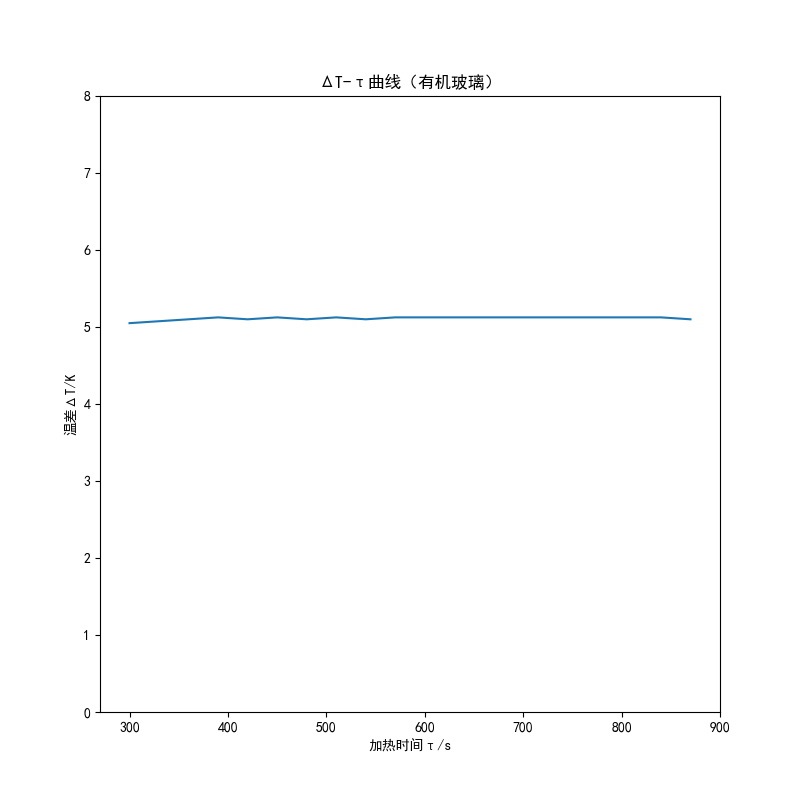
\includegraphics[width=0.9\linewidth]{images/lab9/Figure_1.png}
		\label{chutian1}%文中引用该图片代号
	\end{minipage}
	%\qquad
	\begin{minipage}{0.49\linewidth}
		\centering
		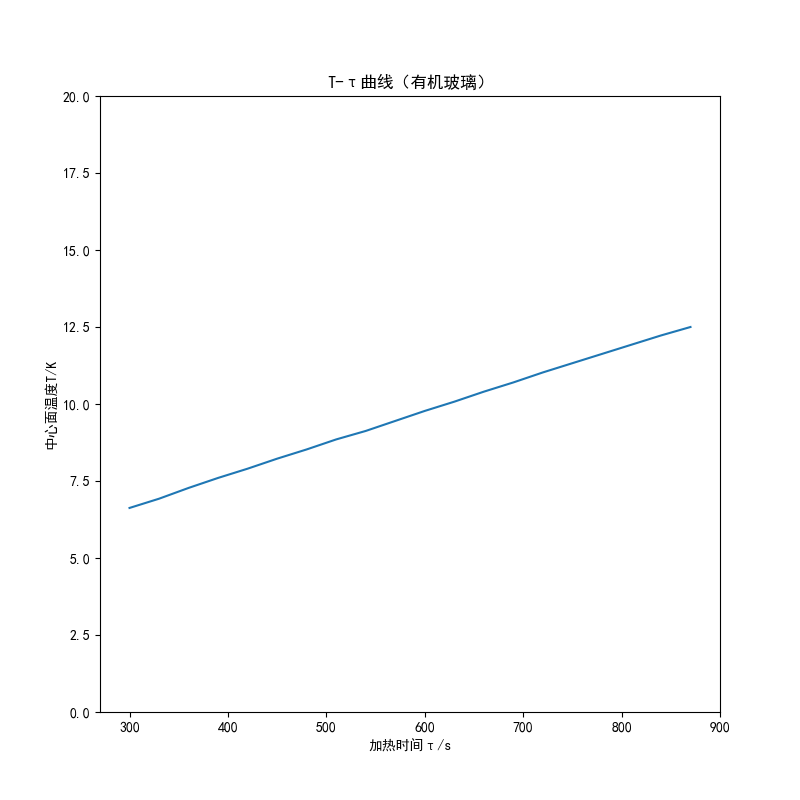
\includegraphics[width=0.9\linewidth]{images/lab9/Figure_2.png}
		\label{chutian2}%文中引用该图片代号
	\end{minipage}
\end{figure}


从图中可看出,加热时间 $τ$ 达到 300s 以后,两个样品的加热面和中心面的温差基本保持不变,且中心面和室
温的温差随时间近似呈线性变化,可视为达到了准稳态。

计算进入准稳态后的 20 组数据的平均值$V_t$,可得

$\Delta T=\frac{V_t}{S}=5.1125K$

$\frac{dT}{d\tau}=\frac{\Delta V}{5*60*S}= 0.29075W/(m \cdot K)$

\subsection{计算有机玻璃样品和橡胶样品的导热系数和比热容。}

热流密度公式  $q_{c}=\frac{A V^{2}}{2 F r}$

导热系数公式  $\lambda=\frac{q_{c} R}{2 \Delta T}$ , 式中  $R=0.010 \mathrm{~m}  $

比热容公式  $c=\frac{q_{c}}{\rho R \frac{\mathrm{d} T}{\mathrm{~d} \tau}} $ 。

根据以上公式和第1问中的  $\Delta T$  和  $\frac{\mathrm{d} T}{\mathrm{~d} \tau}$  数据, 得: 

$ \lambda=0.198 \mathrm{~W} /(\mathrm{m} \cdot \mathrm{K}) $; 

$c=1480 \mathrm{~J} /(\mathrm{kg} \cdot \mathrm{K}) \quad\left(\rho=1196 \mathrm{~kg} / \mathrm{m}^{3}\right) $




\newpage

\section{实验现象分析及结论}

计算得到的有机玻璃样品的导热系数和比热容如下。

$ \lambda=0.198 \mathrm{~W} /(\mathrm{m} \cdot \mathrm{K}) $; 

$c=1480 \mathrm{~J} /(\mathrm{kg} \cdot \mathrm{K}) $

与实际数据有一定差异,可能因为操作不当,测量不准确等原因。

\section{讨论题}



\subsection{本实验中我们采取在样品两端加热的方式根据加热面与中心面的温差及端面温升速率求
出导热系数和比热。实验中为何使用四块样品?}
计算导热系数和比热容时,需要用到热流密度 $q_c$,其通过加热膜的电功率确定。由于加热膜向两面传导热量,若只使用两块样品,热流分布不均,难以计算 $q_c$。实验中采用对称放置四块样品,使得热流均匀分布,简化了热流密度的计算。

\subsection{本实验中判断系统进入准稳态的条件是什么?}

本实验中判断系统进入准稳态的条件是:

1. 加热面与中心面的热电偶电势差保持稳定,即加热面与中心面的温差不变。

2. 中心面与室温的温差呈线性增长,且 $ dT/d\tau $ 保持恒定(因为室温可近似为常数)。

\subsection{本实验中准稳态会无限保持下去吗?是否时间越长实验数据越好?}
本实验中的准稳态不会无限保持。由于实验条件无法完全满足理想模型,随着试样温度升高,边缘效应会加剧,导致温度无法维持理想的准稳态。因此,延长测量时间无助于提高数据质量,实验通常最多持续 35 分钟。

\end{document}